\chapter{Further results}
\label{cha:App-A}

\section{Baseline predictions}

\subsection{Structural time series}
\label{app:structts_preds}
\begin{figure}[H]
	\centering
	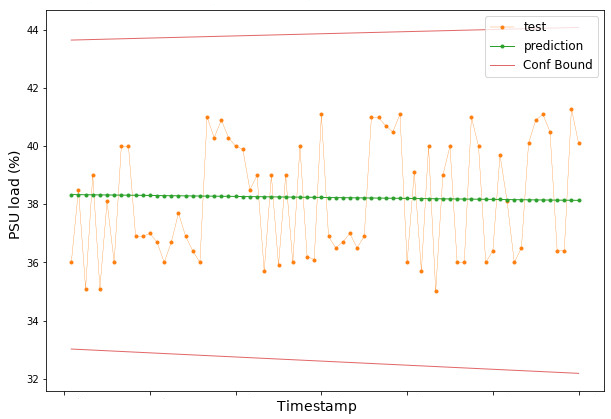
\includegraphics[width=0.8\linewidth]{baseline_imp_preds-sts}
	\caption{Structural model baseline predictions}
	\label{fig:base_sts_preds}
\end{figure}

\begin{figure}[H]
	\centering
	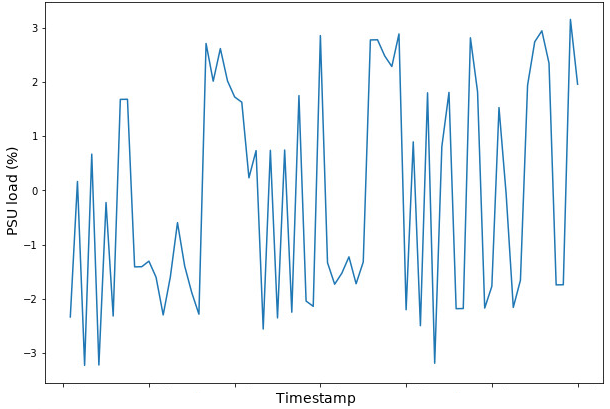
\includegraphics[width=0.8\linewidth]{baseline_imp_residuals-sts}
	\caption{Structural model baseline residuals}
	\label{fig:base_sts_res}
\end{figure}

\subsection{Auto-ARIMA}
\label{app:arima_preds}
\begin{figure}[H]
	\centering
	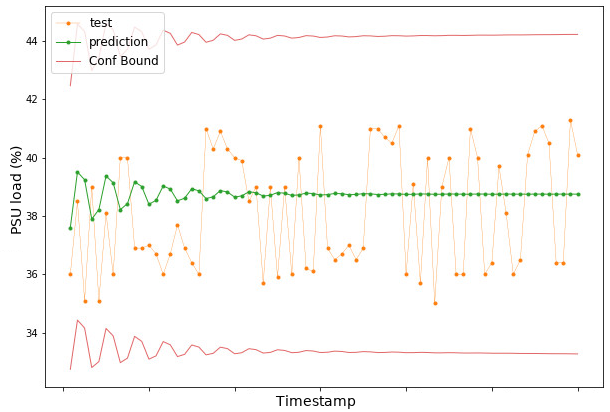
\includegraphics[width=0.8\linewidth]{baseline_imp_preds}
	\caption{Auto-ARIMA baseline predictions}
	\label{fig:base_arima_preds}
\end{figure}

\begin{figure}[H]
	\centering
	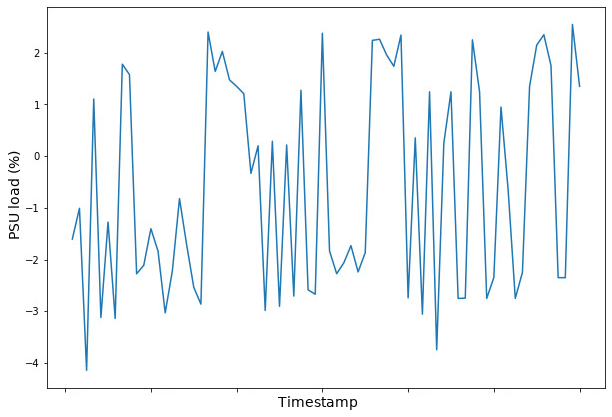
\includegraphics[width=0.8\linewidth]{baseline_imp_residuals}
	\caption{Auto-ARIMA baseline residuals}
	\label{fig:base_arima_res}
\end{figure}



%%%%%%%%%%%%%%%%%%%%%%%%%%%%%%%%%%%%%%%%%%%%%%%%%%%%%%%%%%%%%%%%%%%



\section{Univariate Prophet}
\label{app:uniprophet}


\subsection{Training fitting}

In training is obtained a very poor $R^2$ value, which from the plot in figure \ref{fig:prophet_uni_fitting} can be expected, since $\hat{y}$ looks like mostly an average of the seasonal components. Nonetheless, if it is considered that predicting an interval is acceptable, then the \ac{mobe} shows a very good result. 

It can also be observed that the trend component did not overfit to the outliers.

\begin{table}[H]
	\centering
	\begin{tabular}{|c|c|}
		\hline
		\ac{mae} 	& 2.20 \\
		$R^2$ 		& 0.11 \\
		\ac{mobe} 	& 0.08 \\
		\hline
	\end{tabular}
	\caption{Univariate prophet training scores}
	\label{table:prophet_uni_train_scores}
\end{table}

\begin{figure}[H]
	\centering
	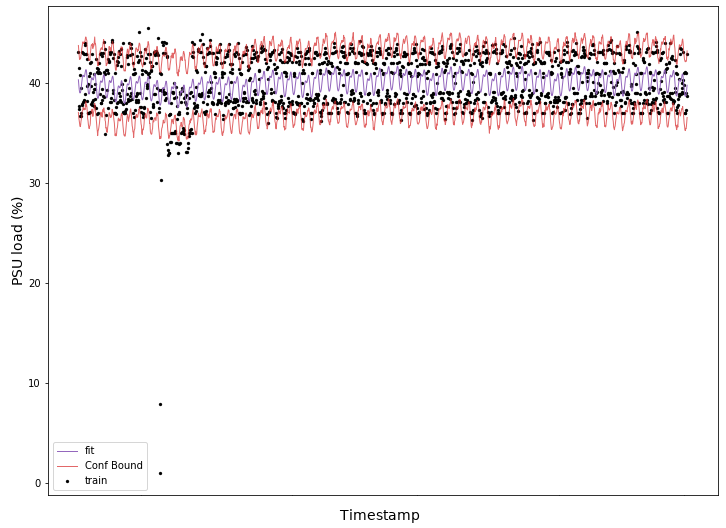
\includegraphics[width=0.8\linewidth]{prophet_uni_fitting}
	\caption{Training fitting from univariate prophet}
	\label{fig:prophet_uni_fitting}
\end{figure}


\subsection{Test predictions}

When it comes to the predictions performance, the $R^2$ shows even worse results. The \ac{mobe} is also high since the trend component was not able to foresee the decreasing in the middle of the test set as shown in Figure \ref{fig:prophet_uni_preds}. 

\begin{figure}[H]
	\centering
	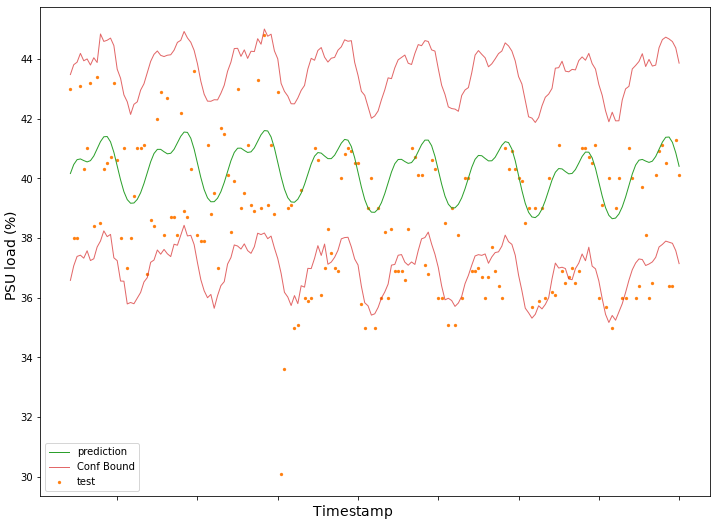
\includegraphics[width=0.8\linewidth]{prophet_uni_preds}
	\caption{Test predictions from the univariate Prophet model}
	\label{fig:prophet_uni_preds}
\end{figure}

\begin{table}[H]
	\centering
	\begin{tabular}{|c|c|}
		\hline
		\ac{mae} 	& 2.12 \\
		$R^2$ 		& -0.33 \\
		\ac{mobe} 	& 0.25 \\
		\hline
	\end{tabular}
	\caption{Univariate prophet prediction performance}
	\label{table:prophet_uni_test_scores}
\end{table}

\subsection{Residual analysis}

The residuals in the training set still show somehow resembles the original data pattern. This could be interpreted that there is still patterns to learn from data, i.e., this model is not complete. 

\begin{figure}[hptb]
	\centering
	\begin{subfigure}{.8\textwidth}
		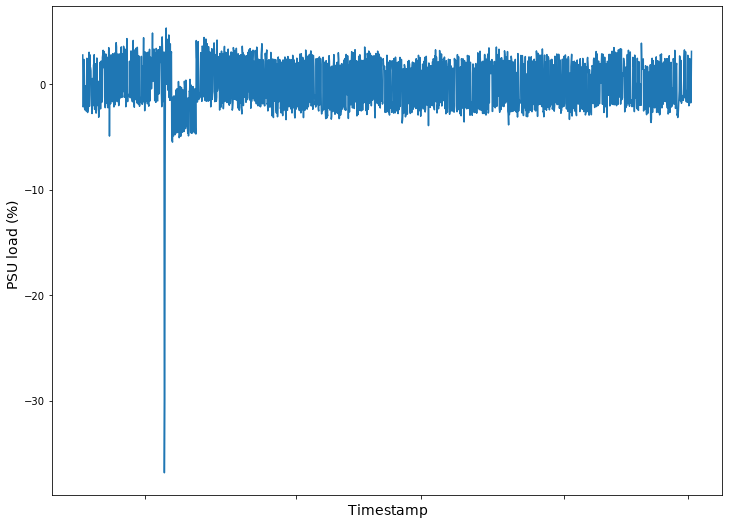
\includegraphics[width=\textwidth]{prophet_train_res_time}
		\caption{Residuals from train fit}
		\label{fig:prophet_train_res_time}
	\end{subfigure}%
	\hfill
	\begin{subfigure}{.8\textwidth}
		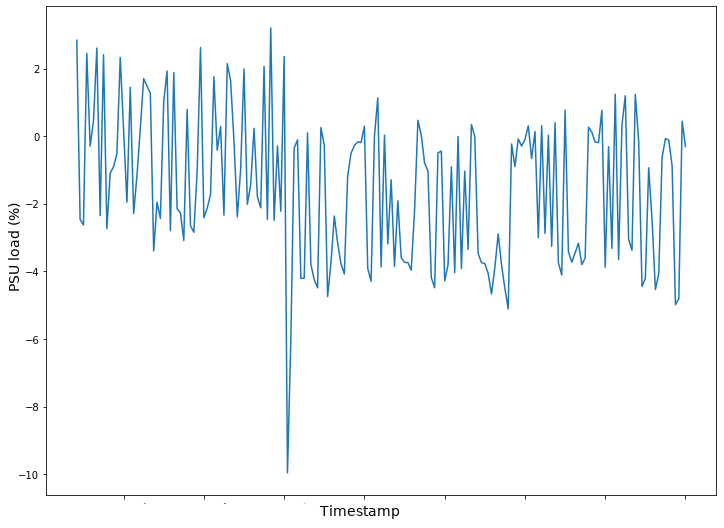
\includegraphics[width=\textwidth]{prophet_test_res_time}
		\caption{Residuals from test predictions}
		\label{fig:prophet_test_res_time}
	\end{subfigure}
	\caption{Univariate prophet residuals}
	\label{fig:prophet_res_time}
\end{figure}



%%%%%%%%%%%%%%%%%%%%%%%%%%%%%%%%%%%%%%%%%%%%%%%%%%%%%%%%%%%%%%%%%%%



\section{Multivariate Prophet}

\subsection{Test predictions}

The results of the predictions have notoriously improved in this case. The $R^2$ value is close to 0.9, which for such a complex signal shows how powerful is the model. 

The \ac{mobe} has even decreased in the test set, this could be due to training outliers that still being difficult to approximate without overfitting the trend component. 


\begin{table}[H]
	\centering
	\begin{tabular}{|c|c|}
		\hline
		\ac{mae} 	& 0.52 \\
		$R^2$ 		& 0.88 \\
		\ac{mobe} 	& 0.05 \\
		\hline
	\end{tabular}
	\caption{Multivariate prophet prediction performance}
	\label{table:prophet_multi_test_scores}
\end{table}



\begin{figure}[H]
	\centering
	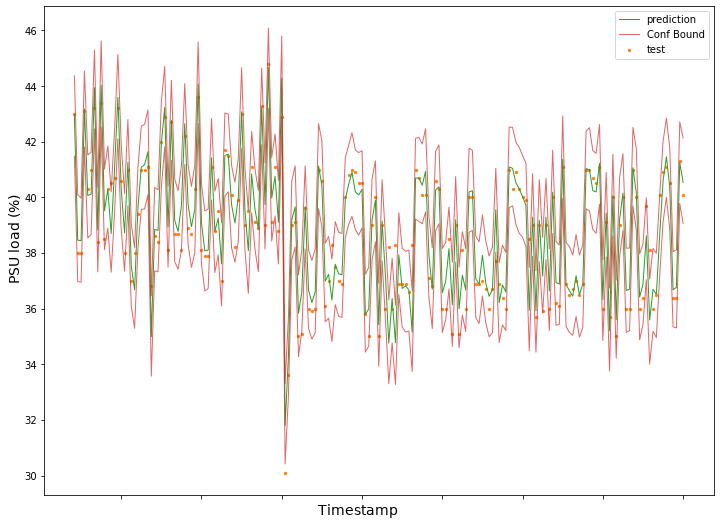
\includegraphics[width=0.6\linewidth]{prophet_multi_preds}
	\caption{Test predictions from multivariate prophet}
	\label{fig:prophet_multi_preds}
\end{figure}


\subsection{Residual analysis}

The residuals show that the patterns have been better learnt than in the univariate case.

\begin{figure}[hptb]
	\centering
	\begin{subfigure}{.8\textwidth}
		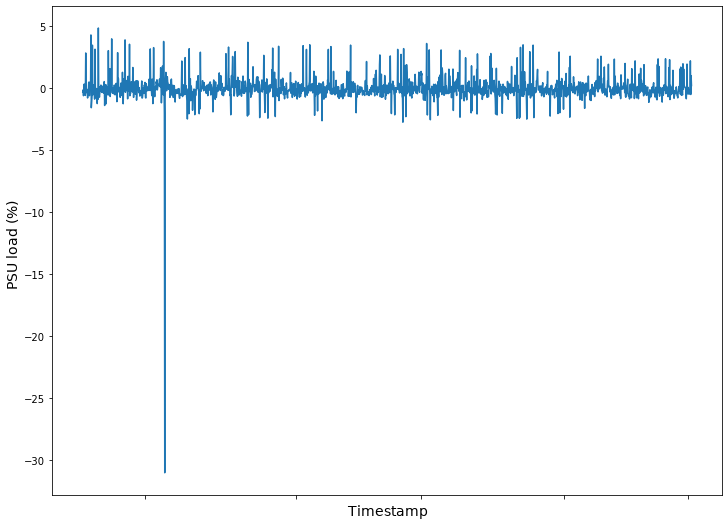
\includegraphics[width=\textwidth]{prophet_train_res_time_multi}
		\caption{Train}
		\label{fig:prophet_train_res_time_multi}
	\end{subfigure}%
	\hfill
	\begin{subfigure}{.8\textwidth}
		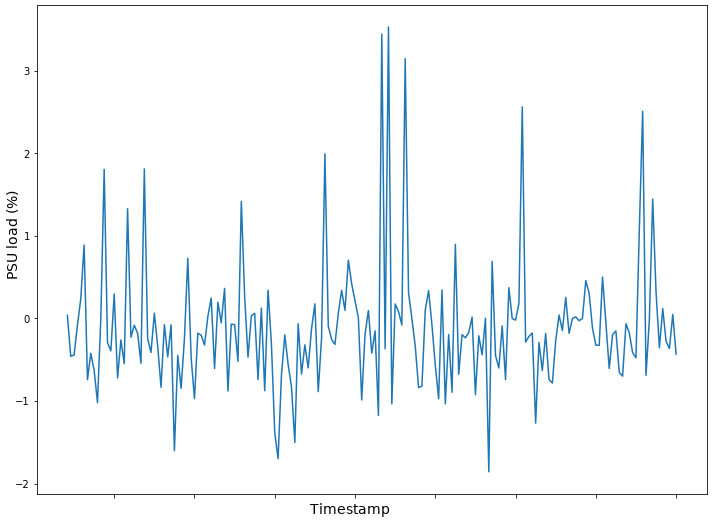
\includegraphics[width=\textwidth]{prophet_test_res_time_multi}
		\caption{Test}
		\label{fig:prophet_test_res_time_multi}
	\end{subfigure}
	\caption{Multivariate prophet residuals}
	\label{fig:prophet_res_time_multi}
\end{figure}


%%%%%%%%%%%%%%%%%%%%%%%%%%%%%%%%%%%%%%%%%%%%%%%%%%%%%%%%%

\section{Exhaustive experiments}

\subsection{Baselines predictions moving horizon}

\begin{figure}[H]
	\centering
	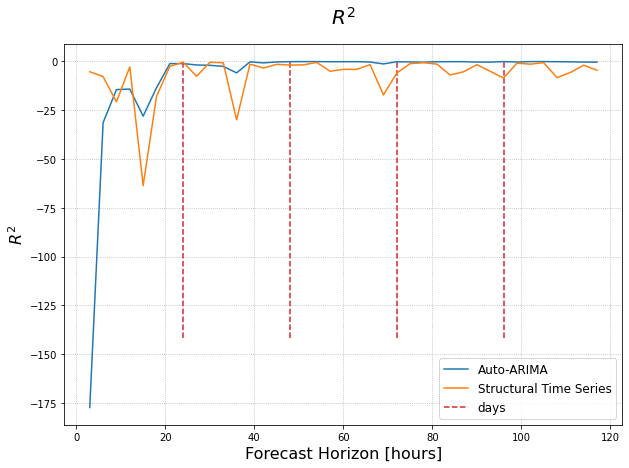
\includegraphics[width=0.8\linewidth]{baseline_db-structts_R2}
	\caption{Baseline $R^2$}
	\label{fig:baseline_structts_r2}
\end{figure}

\begin{figure}[H]
	\centering
	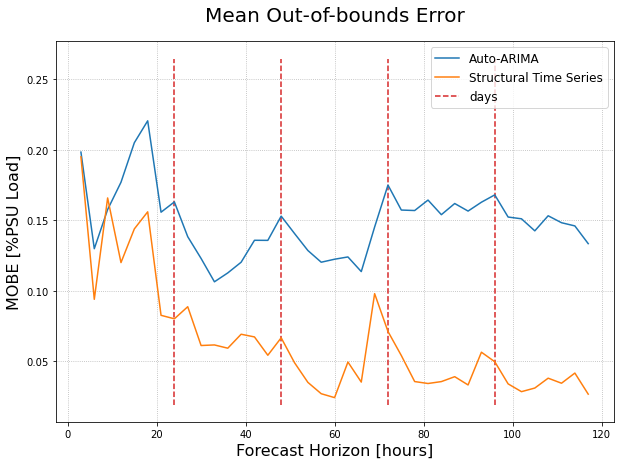
\includegraphics[width=0.8\linewidth]{baseline_db-structts_MOBE}
	\caption{Baseline MOBE}
	\label{fig:baseline_structts_mobe}
\end{figure}




\subsection{Univariate Prophet prediction moving horizon}

\begin{figure}[H]
	\centering
	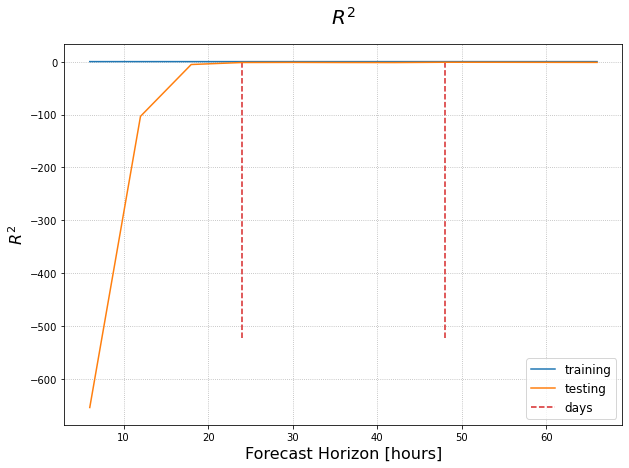
\includegraphics[width=0.8\linewidth]{exp_prophet_uni_r2_time}
	\caption{Univariate moving prediction horizon: $R^2$}
	\label{fig:exp_prophet_uni_r2}
\end{figure}

\begin{figure}[H]
	\centering
	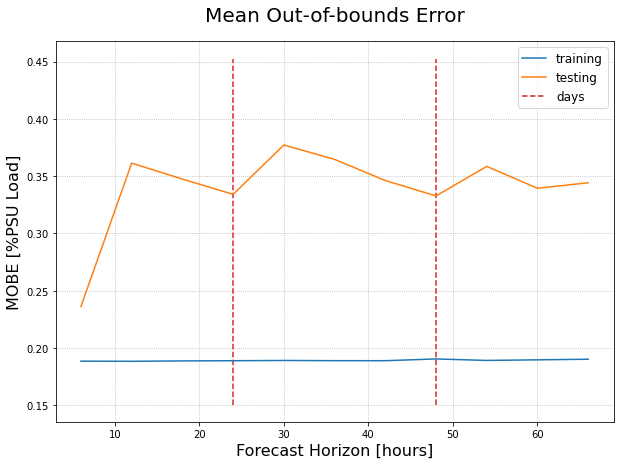
\includegraphics[width=0.8\linewidth]{exp_prophet_uni_mobe_time}
	\caption{Univariate moving prediction horizon: \ac{mobe}}
	\label{fig:exp_prophet_uni_mobe}
\end{figure}

\subsection{Multivariate Prophet prediction moving horizon}





\begin{figure}[H]
	\centering
	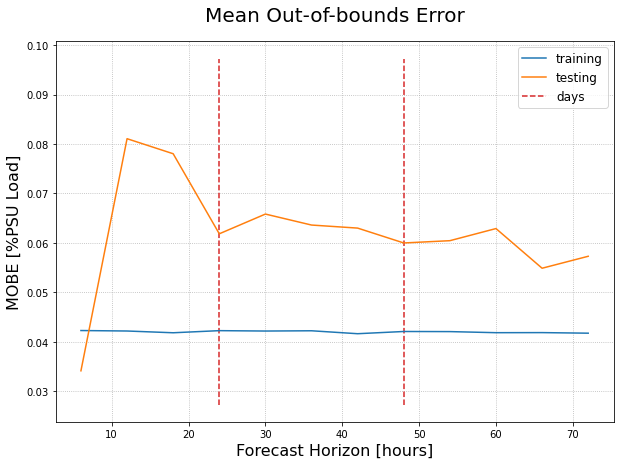
\includegraphics[width=0.8\linewidth]{exp_prophet_mv_mobe_time}
	\caption{Multivariate moving prediction horizon: \ac{mobe}}
	\label{fig:exp_prophet_mv_mobe}
\end{figure}











